% =============================================================================
%  One-page Research Paper Summary
%  Single-file standalone. Optional logo: ABV_IIITM_Logo.jpeg.
% =============================================================================
\documentclass[9pt,a4paper]{extarticle}

\usepackage[utf8]{inputenc}
\usepackage[T1]{fontenc}
\usepackage{lmodern}
\usepackage[a4paper,margin=0.45in,top=0.4in,bottom=0.4in]{geometry}
\usepackage{amsmath,amssymb}
\usepackage{booktabs}
\usepackage{xcolor}
\usepackage{enumitem}
\usepackage{multicol}
\usepackage{graphicx}
\usepackage{tikz}
\usetikzlibrary{shapes.geometric, arrows.meta, positioning, calc}
\usepackage[hidelinks]{hyperref}

\definecolor{iiitmblue}{RGB}{12,42,86}
\definecolor{accentred}{RGB}{180,30,30}

\setlength{\parindent}{0pt}
\setlength{\parskip}{1pt}
\linespread{0.96}
\pagestyle{empty}

\renewcommand{\section}[1]{%
  \par\vspace{1pt}%
  \noindent{\color{iiitmblue}\bfseries #1}%
  \vspace{0.5pt}\hrule height 0.4pt%
  \par\vspace{1pt}%
}

\begin{document}

% ---------- Header ----------
\begin{minipage}[c]{0.78\textwidth}
\raggedright
{\Large\bfseries Reducing Cross-Node Network Calls in Distributed Payment Systems via Thread-Level and Server-Local Caching}\\[2pt]
{\itshape with Concurrency-Safe Resolution of Single-Resource Contention}\\[3pt]
{\small Raman Kapoor \,$\bullet$\, Supervisor: Dr.\ Vivek Kumar Singh \,$\bullet$\, ABV-IIITM Gwalior \,$\bullet$\, B.Tech (IT) End-Term, 2026}
\end{minipage}\hfill
\begin{minipage}[c]{0.18\textwidth}
\raggedleft
\IfFileExists{ABV_IIITM_Logo.jpeg}{
\includegraphics[height=1.7cm]{ABV_IIITM_Logo.jpeg}}{}
\end{minipage}

\vspace{4pt}\hrule height 1pt
\vspace{4pt}

% ---------- Abstract ----------
{\footnotesize
Production payment APIs face two intertwined hazards: redundant cross-node lookups inflate p95/p99 tail latency, and concurrent operations on \emph{single, indivisible} resources (last inventory unit, unique reservation slot, account debit) can be \textbf{double-allocated} when caching introduces stale reads. This work integrates a two-tier in-process cache (governed by formal safety boundaries) with a \textbf{contention layer} of five complementary primitives that closes every variant of the double-booking race. Production at $\sim$68{,}000 cross-node ops/sec: \textbf{--11.2\,\% p95 latency}, \textbf{4.1\,\% network reduction}, \textbf{zero double-allocation incidents} over 30 days.
}

% ---------- The double-booking question ----------
\section{The Double-Booking Question}

The minor evaluation surfaced the central question this paper answers:
\emph{``If you cache state, how do you prevent two users from booking the same single piece?''}

\begin{minipage}[t]{0.50\textwidth}
\vspace{0pt}
\textbf{The hazard.} Two concurrent requests $R_1$ and $R_2$ each read a cached \texttt{stock = 1}, both pass the availability check, both decrement on the backend $\Rightarrow$ \texttt{stock = -1}, two customers receive the same unit. Caching that satisfies the four cache-safety boundaries (immutability within TTL, request-scope independence, idempotency of stale reads, deterministic key) is correct for \emph{configuration-class} data --- but \emph{single-resource state fails criterion (3) by construction}: a stale read produces a financial discrepancy. Such state is therefore explicitly excluded from the cache and routed through the contention layer.
\end{minipage}\hfill
\begin{minipage}[t]{0.46\textwidth}
\vspace{0pt}
\centering
\resizebox{\linewidth}{!}{%
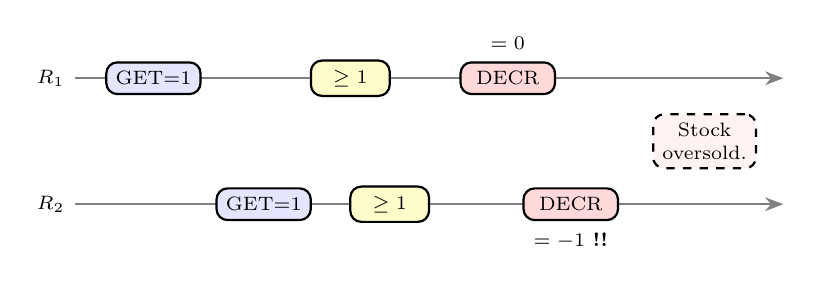
\begin{tikzpicture}[>=Stealth, thick, every node/.style={font=\scriptsize}]
  \draw[->, gray] (0,1.6) -- (9,1.6); \draw[->, gray] (0,0) -- (9,0);
  \node[left] at (0,1.6) {$R_1$}; \node[left] at (0,0) {$R_2$};
  \node[draw, fill=blue!10, rounded corners, minimum width=1.1cm] (a) at (1.0,1.6) {GET=1};
  \node[draw, fill=blue!10, rounded corners, minimum width=1.1cm] (b) at (2.4,0)  {GET=1};
  \node[draw, fill=yellow!20, rounded corners, minimum width=1.0cm] at (3.5,1.6) {$\geq 1$};
  \node[draw, fill=yellow!20, rounded corners, minimum width=1.0cm] at (4.0,0)  {$\geq 1$};
  \node[draw, fill=red!15, rounded corners, minimum width=1.2cm]    (d) at (5.5,1.6) {DECR};
  \node[draw, fill=red!15, rounded corners, minimum width=1.2cm]    (e) at (6.3,0)  {DECR};
  \node[font=\scriptsize, above=0.02cm of d] {$=0$};
  \node[font=\scriptsize, below=0.02cm of e] {$=-1$ \textbf{!!}};
  \node[draw, dashed, fill=red!5, rounded corners, align=center, font=\scriptsize] at (8.0,0.8) {Stock\\oversold.};
\end{tikzpicture}}
\\\textit{Lost-update race on a single-resource decrement.}
\end{minipage}

% ---------- Five primitives ----------
\section{Contention Layer --- Five Complementary Primitives}

\begin{multicols}{2}
\small
\begin{enumerate}[leftmargin=1.1em, itemsep=2pt]
  \item \textbf{Distributed lock + fencing token} (Redlock / etcd lease). Per-resource lock; backend rejects writes with stale tokens. Use for non-trivial logic with external calls. \emph{+1--3\,ms; caps per-key throughput.}
  \item \textbf{Atomic decrement via Redis Lua.} Bundle ``check $\geq 1$ + decrement'' in one Lua script; Redis runs it serialised. Use for hard-limit inventory and reservations. \emph{$<$1\,ms; $>10^5$ scripts/s/shard.}
  \item \textbf{Optimistic concurrency (OCC) with versioned cache.} Reader records version; writer issues a CAS update conditioned on it. Use only when conflicts are \emph{rare} (e.g., control-plane writes); under high contention, retry storms collapse throughput.
  \item \textbf{PN-Counter CRDT.} Two grow-only counters per replica; merge by element-wise max. Use only when over-allocation is \emph{business-acceptable} (soft holds, cart counters). 4.7 over-allocations / day on 100k base.
  \item \textbf{Single-flight request coalescing.} On a cache miss, only the first concurrent request fetches; the rest share its result. \emph{Not} a replacement for atomicity --- always paired with one of (1)--(4).
\end{enumerate}
\end{multicols}

% ---------- Decision matrix ----------
\section{Decision Matrix \& Hybrid Architecture}

\begin{minipage}[t]{0.62\textwidth}
\vspace{0pt}
\footnotesize
\setlength{\tabcolsep}{4pt}
\renewcommand{\arraystretch}{1.05}
\begin{tabular}{p{2.6cm}p{1.2cm}p{2.0cm}p{2.0cm}}
\toprule
\textbf{Data class} & \textbf{Cache?} & \textbf{Primary} & \textbf{Coalescing} \\
\midrule
Merchant config (read)   & Tier-2 & ---              & Single-flight \\
Inventory (display)      & Tier-2 & ---              & Single-flight \\
Inventory (decrement)    & No     & Lua atomic       & Single-flight \\
Account balance debit    & No     & Distributed lock & Single-flight \\
Reservation slot         & No     & Lua atomic       & Single-flight \\
Soft hold (cart)         & Tier-2 & PN-Counter       & ---           \\
Merchant config (write)  & Inval. & OCC versioned    & ---           \\
\bottomrule
\end{tabular}
\end{minipage}\hfill
\begin{minipage}[t]{0.34\textwidth}
\vspace{0pt}
\small
\textbf{Hybrid flow.} \emph{Reads} traverse Tier-1 (thread cache) $\to$ single-flight $\to$ Tier-2 (server cache) $\to$ Redis. \emph{Authoritative writes} bypass the cache and select a primitive per Table; on success they publish a Pub/Sub invalidation that propagates to Tier-2 within tens of milliseconds. Single-flight is always layered in front of cache misses to absorb thundering-herd amplification.
\end{minipage}

% ---------- Results ----------
\section{Production Results (30-day window, $\sim$68{,}000 cross-node ops/sec)}

\begin{minipage}[t]{0.49\textwidth}
\vspace{0pt}
\small
\textbf{Phase 1 --- Caching only:}
\begin{itemize}[leftmargin=1.1em, itemsep=0pt, topsep=2pt]
  \item Combined hit rate: \textbf{54.8\,\%} on eligible lookups
  \item Cross-node calls eliminated: $\sim$2{,}800/s ($\downarrow$ \textbf{4.1\,\%})
  \item p95 API latency: 98 $\to$ 87\,ms (\textbf{--11.2\,\%})
  \item p99 API latency: 285 $\to$ 248\,ms (\textbf{--13.0\,\%})
  \item Redis p99 latency: 12.5 $\to$ 9.2\,ms (\textbf{--26.2\,\%})
  \item Memory overhead per node: $<$20\,MB
\end{itemize}
\end{minipage}\hfill
\begin{minipage}[t]{0.49\textwidth}
\vspace{0pt}
\small
\textbf{Phase 2 --- Contention layer:}
\begin{itemize}[leftmargin=1.1em, itemsep=0pt, topsep=2pt]
  \item Inventory decrement (flash sale): 1{,}400/s contended, +0.8\,ms p95 (Lua + single-flight)
  \item Per-merchant settlement: 12/s contended, +2.6\,ms p95 (Lock + fence)
  \item Reservation slot: 320/s contended, +1.1\,ms p95 (Lua)
  \item \textbf{Zero} double-allocation incidents
  \item \textbf{Zero} cache-related financial discrepancies
\end{itemize}
\end{minipage}

\vspace{4pt}
\hrule height 0.4pt
\vspace{2pt}
\centering\footnotesize\itshape
The minor's question --- ``how do we prevent two users from booking the same single piece?'' --- is answered, end-to-end, by the contention layer.

\end{document}
